\subsection{Очищаем сигнал}

Итак, для начала строим график исходного сигнала:

\begin{figure}[ht!]
    \centering
    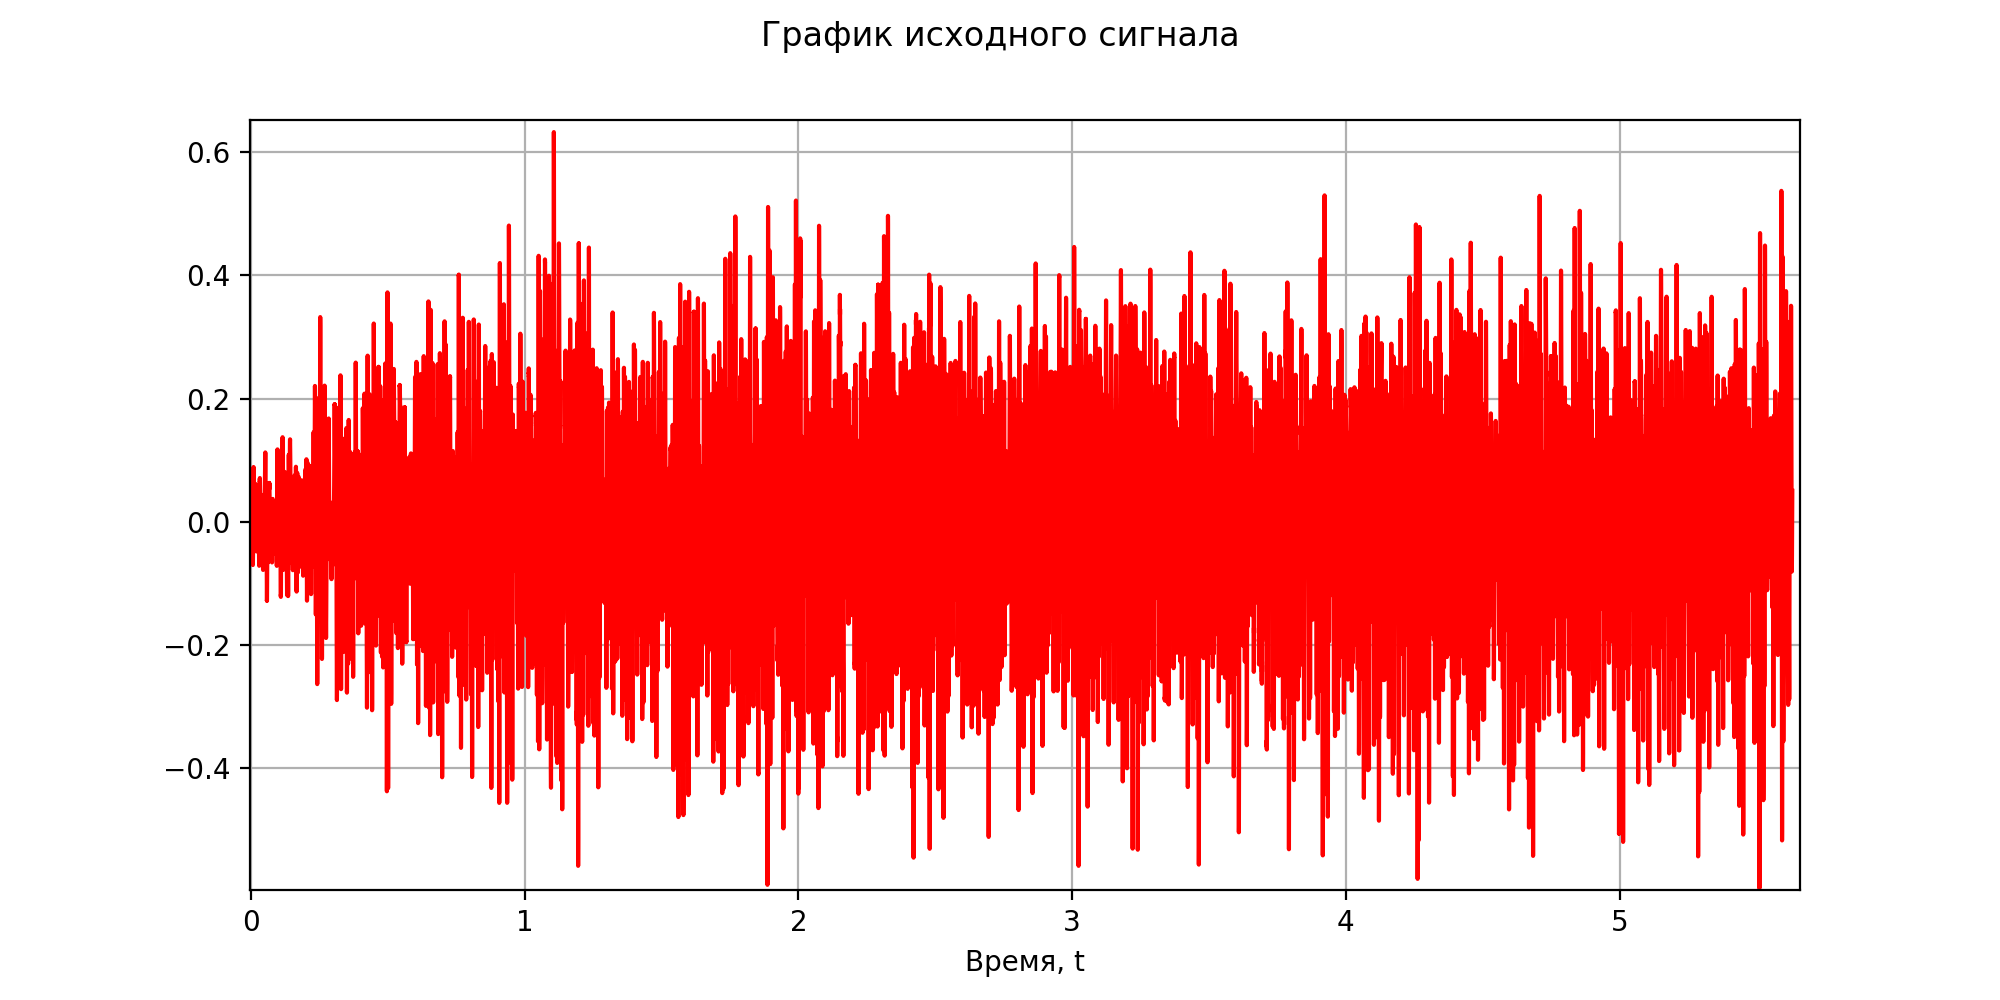
\includegraphics[scale=0.5]{media/2 task/Source_Звуковая волна.png}
    \caption{График исходной звуковой волны}
    \label{fig:initial_wave}
\end{figure}

Довольно много шума, согласны? Поэтому переходим к Фурье-образу нашей аудиозаписи (в данном задании использовалось Фурье-преобразование по угловой частоте):

\begin{figure}[ht!]
    \centering
    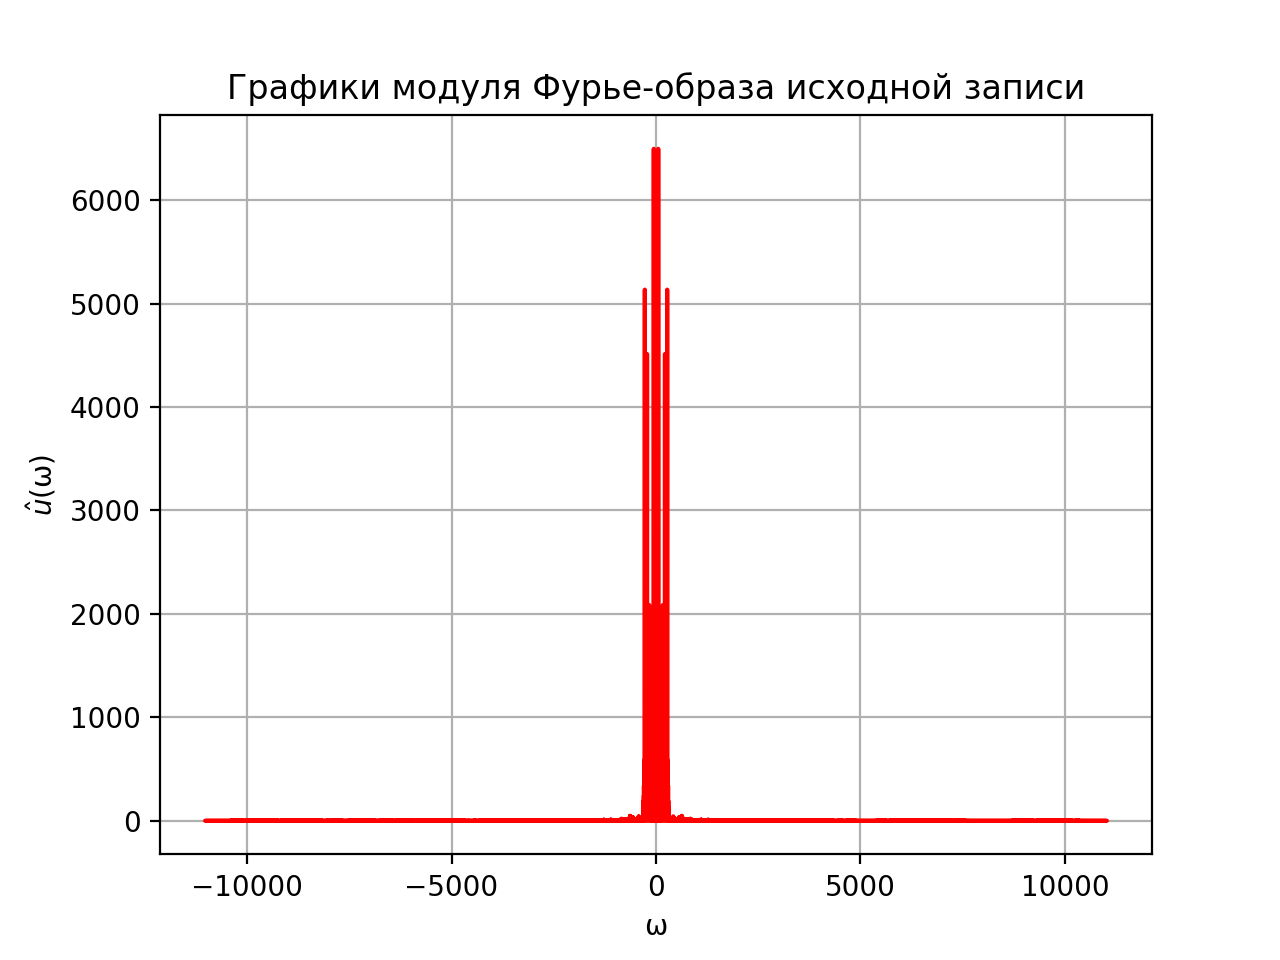
\includegraphics[scale=0.6]{media/2 task/Image_Orig.png}
    \caption{График модуля Фурье-образа исходной волны}
    \label{fig:four_orig_wave}
\end{figure}

\clearpage

Очевидно, что для анализа нам нужно рассмотреть график на промежутке $\omega \in [-400, 400]$ $\frac{\text{рад}}{\text{с}}$:

\begin{figure}[ht!]
    \centering
    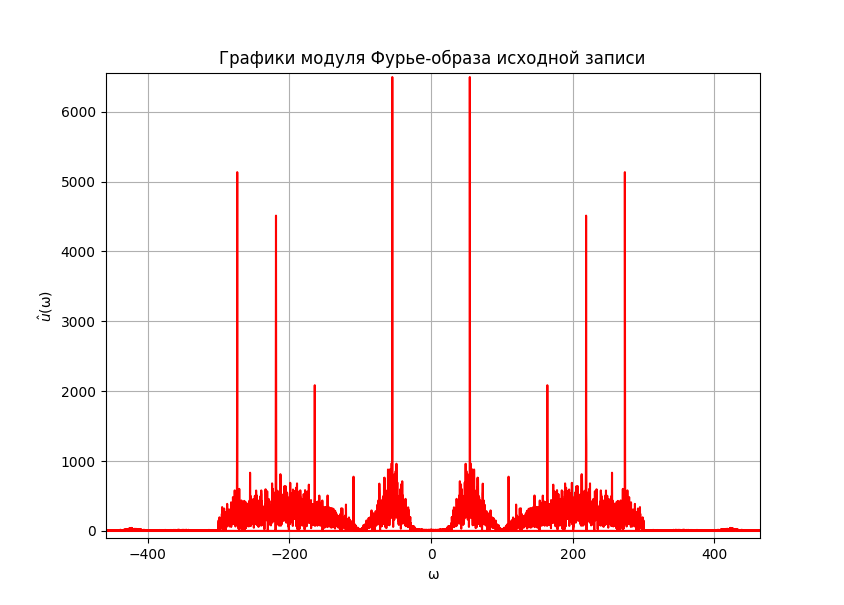
\includegraphics[width=\textwidth]{media/2 task/Image_CLose.png}
    \caption{График модуля Фурье-образа исходной волны на промежутке $\omega \in [-400, 400]$ $\frac{\text{рад}}{\text{с}}$}
    \label{fig:four_orig_detailed_wave}
\end{figure}

При прослушивании аудиозаписи были замечены 2 вида шума: гул (низкочастотный шум) и щебетание птиц (высокочастотный шум). Для начала разберёмся с первыми помехами. Попробуем обнулить все частоты в диапазоне $\omega \in [-300, 300]$ $\frac{\text{рад}}{\text{с}}$. Для исключения птичьего щебетания эмперическим путём было выявлено, что нужно отбросить все частоты выше $4500$ $\frac{\text{рад}}{\text{с}}$. Полученные графики:

\begin{figure}[ht!]
    \centering
    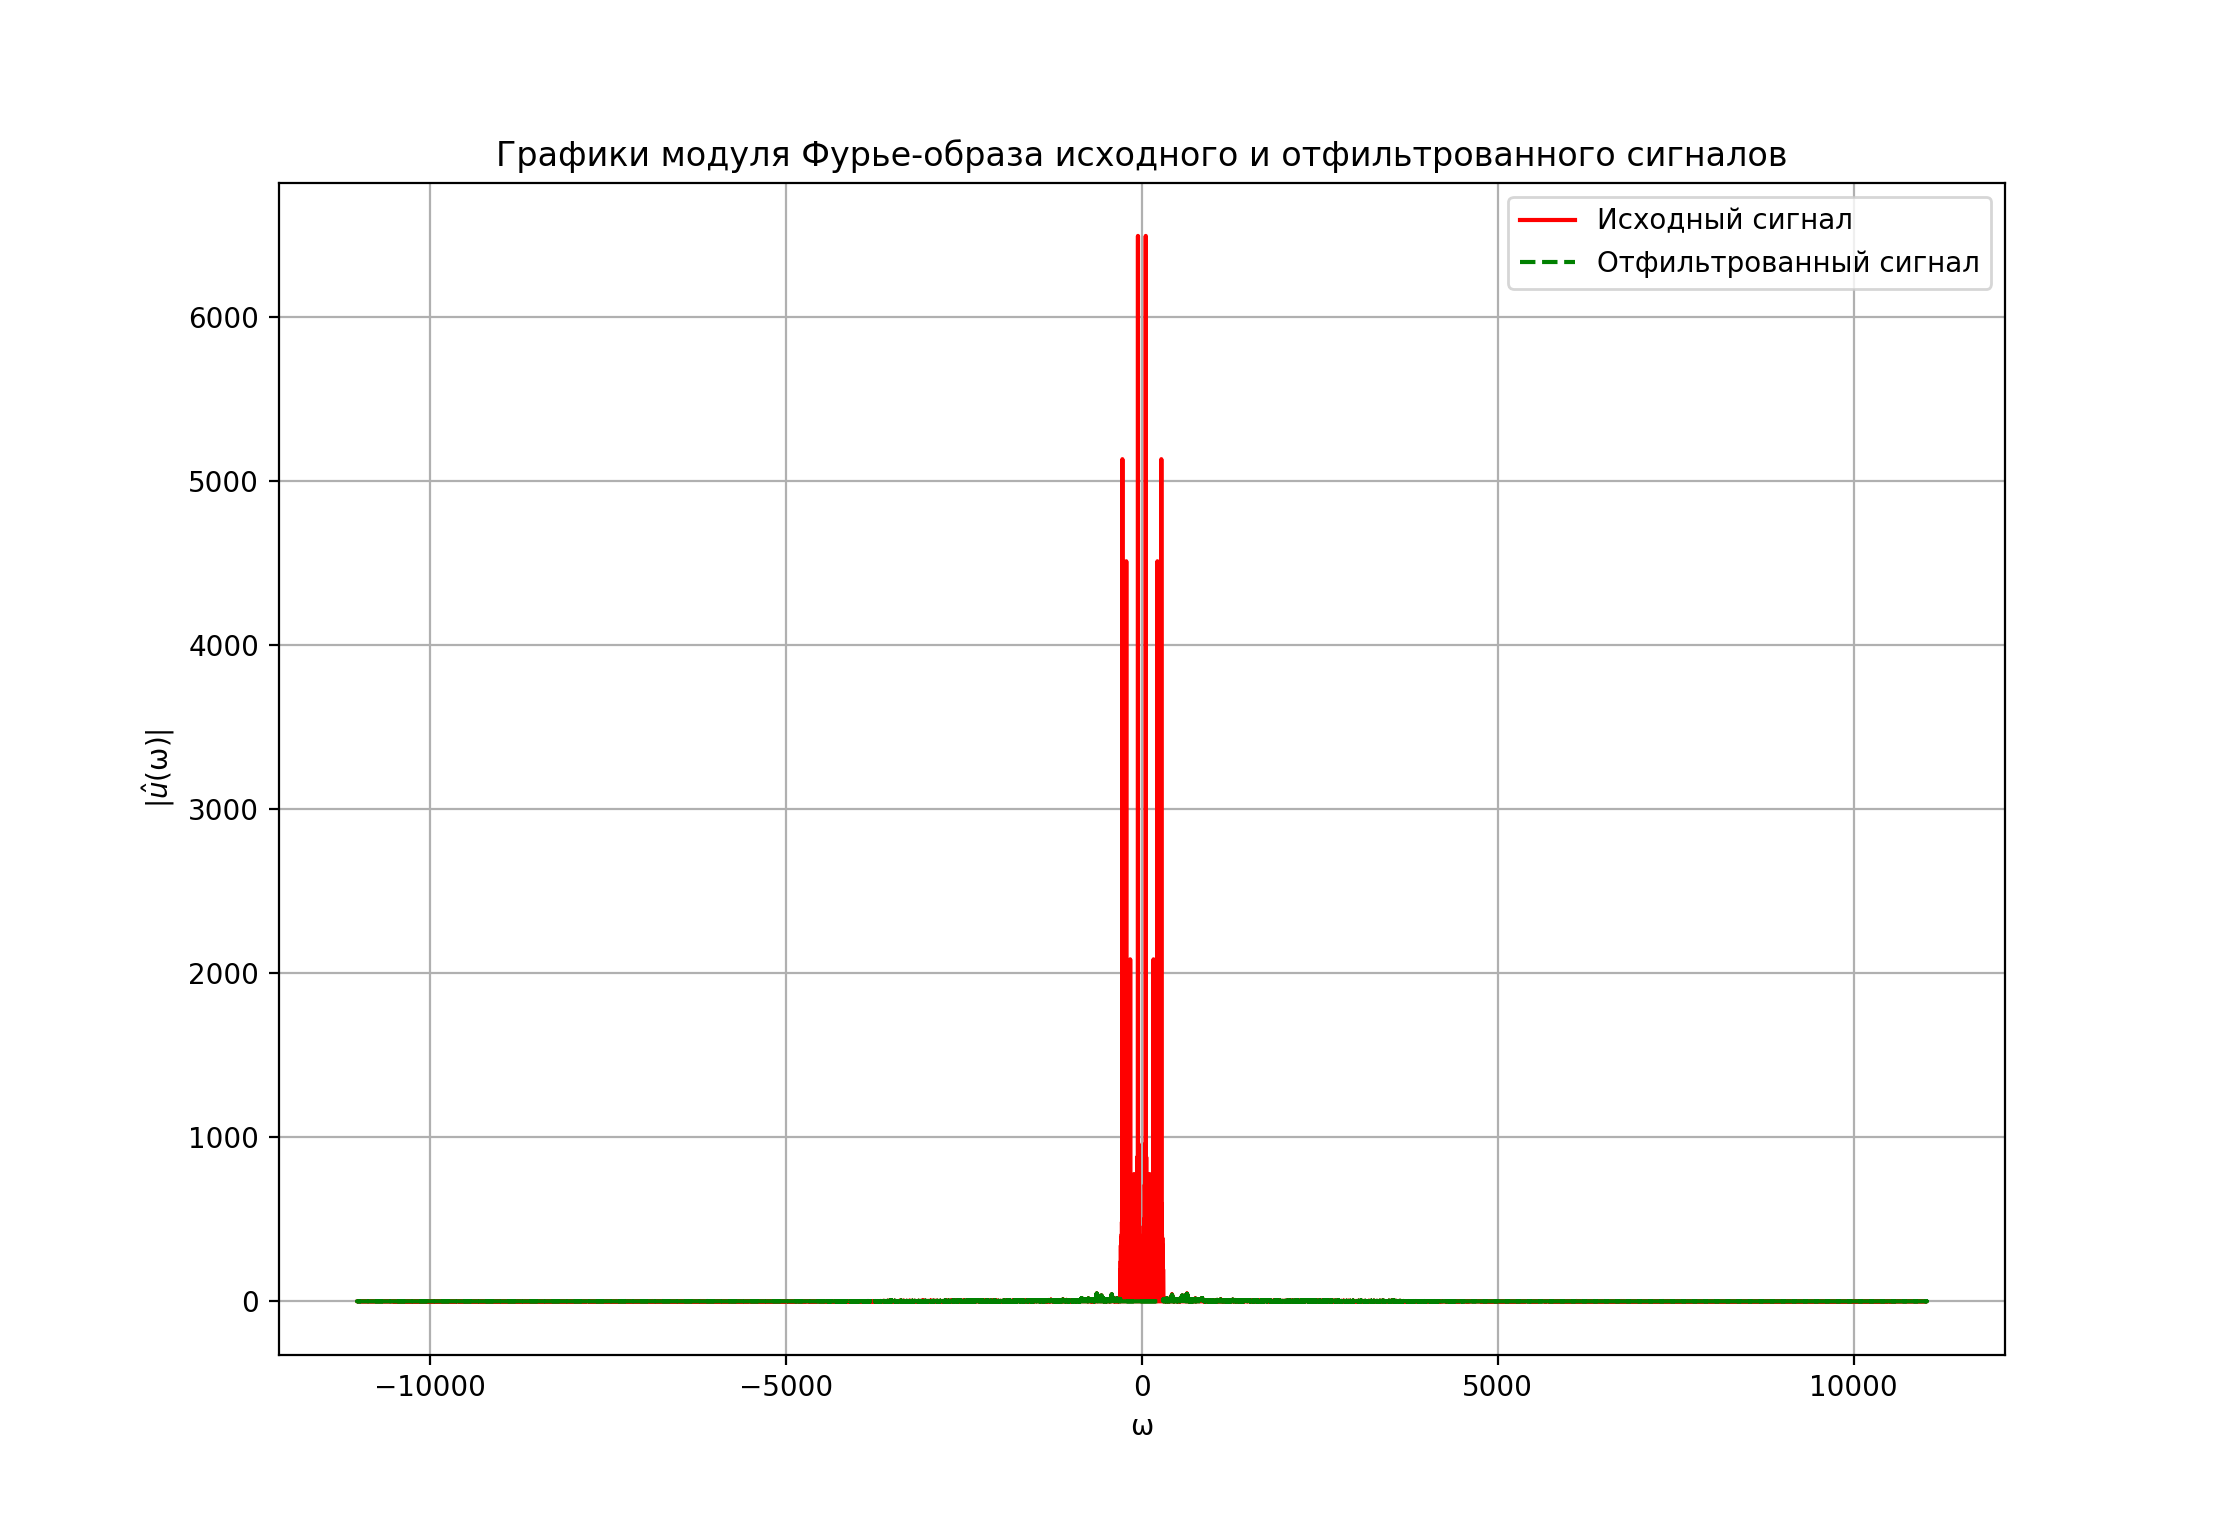
\includegraphics[width=\textwidth]{media/2 task/Images_Comparison.png}
    \caption{Сравнительные графики модулей Фурье-образов исходной и отфильтрованной аудиозаписей}
    \label{fig:fourc_orig_wave}
\end{figure}

\begin{figure}[ht!]
    \centering
    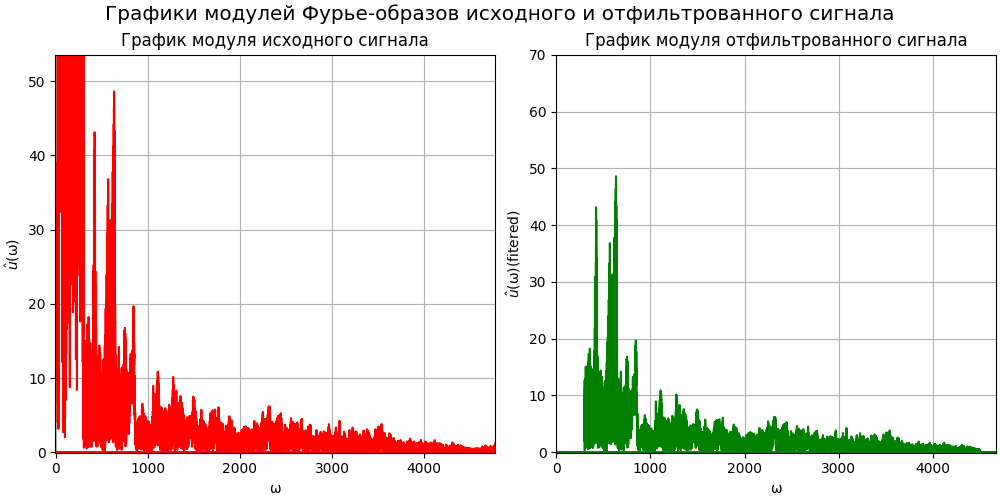
\includegraphics[width=\textwidth]{media/2 task/detailed_comparison.png}
    \caption{Графики модулей Фурье-образов исходной и отфильтрованной аудиозаписей на промежутке $\omega \in [0, 5000]$ $\frac{\text{рад}}{\text{с}}$}
    \label{fig:fourc_orig_detailed_wave}
\end{figure}

\clearpage
\subsection{Наслаждаемся результатом!}

В результате мы получили аудиозапись (\href{https://disk.yandex.ru/d/NHTrsfW_m_KmMQ}{ссылка}), на которой отчётливо слышен голос и отсутствуют вышеупомянутые шумы.

График фильтрованной функции:

\begin{figure}[ht!]
    \centering
    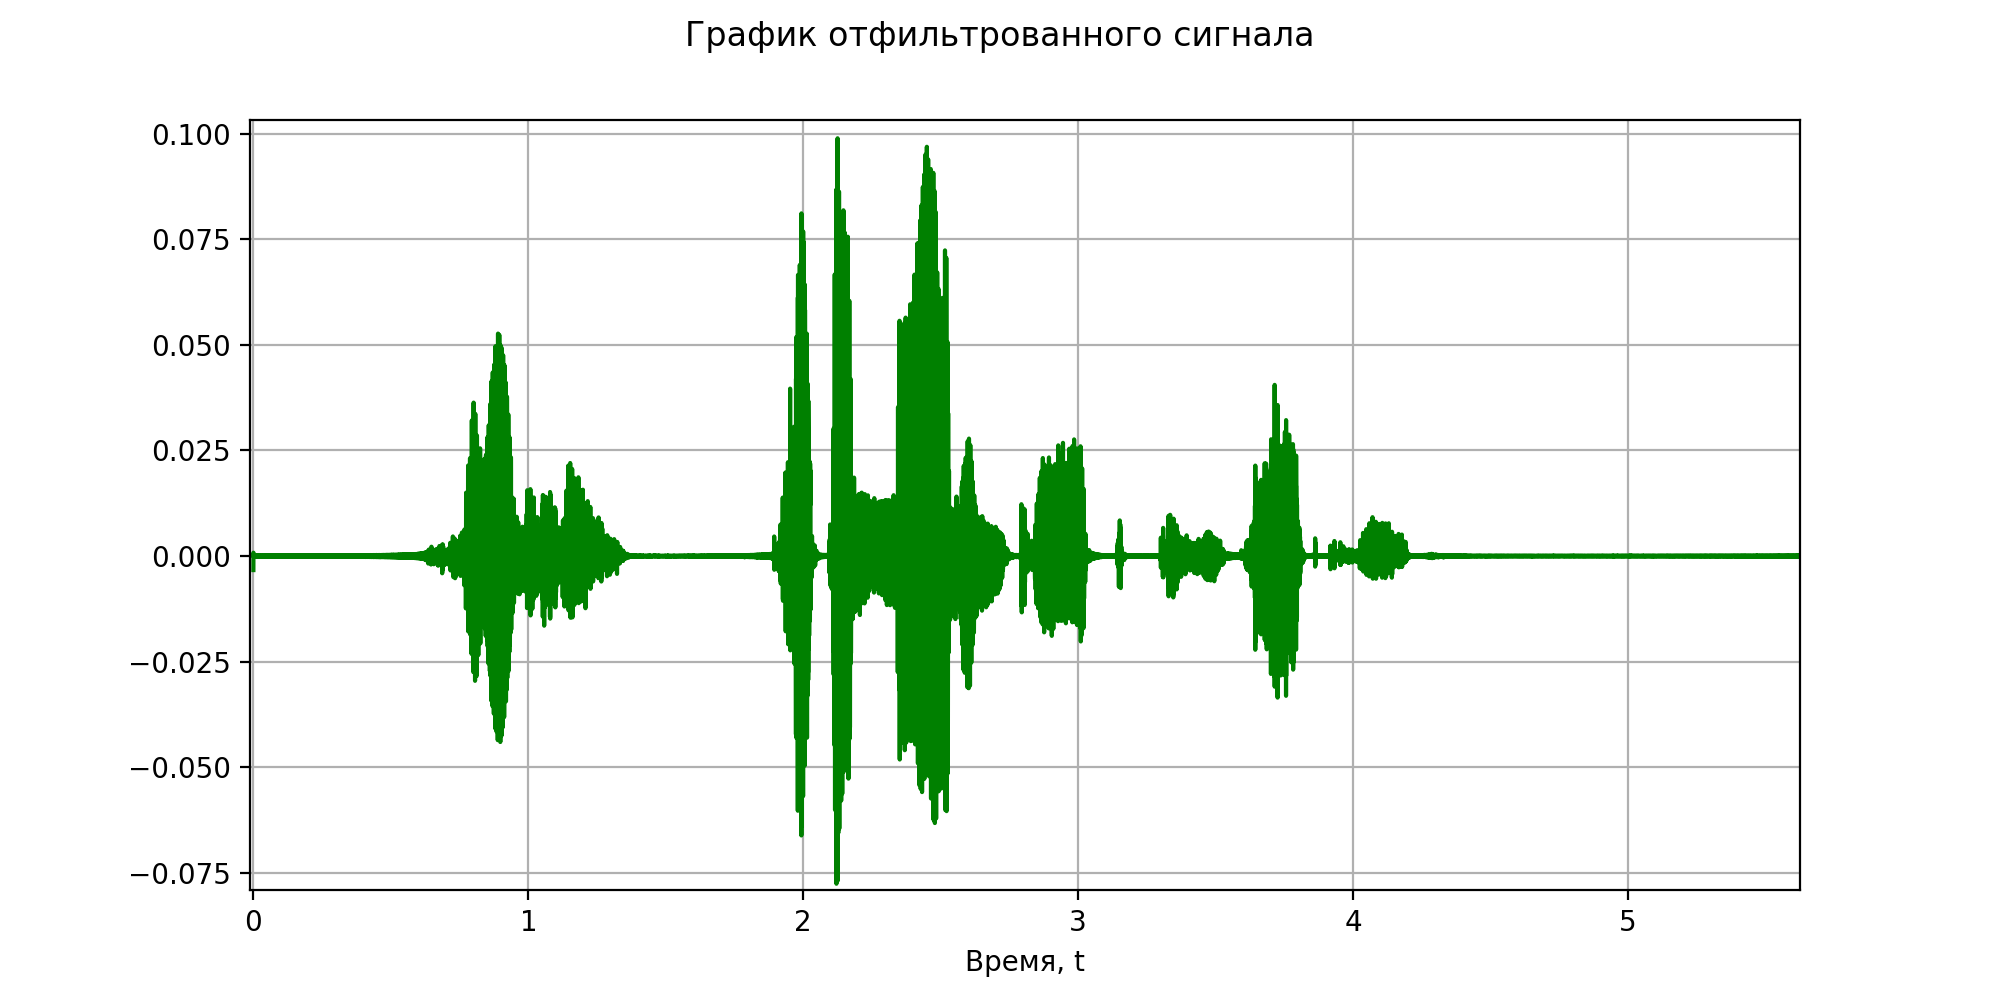
\includegraphics[scale=0.6]{media/2 task/Cleaned_Звуковая волна.png}
    \caption{График отфильтрованной звуковой волны}
    \label{fig:filtered_wave}
\end{figure}

\begin{figure}[ht!]
    \centering
    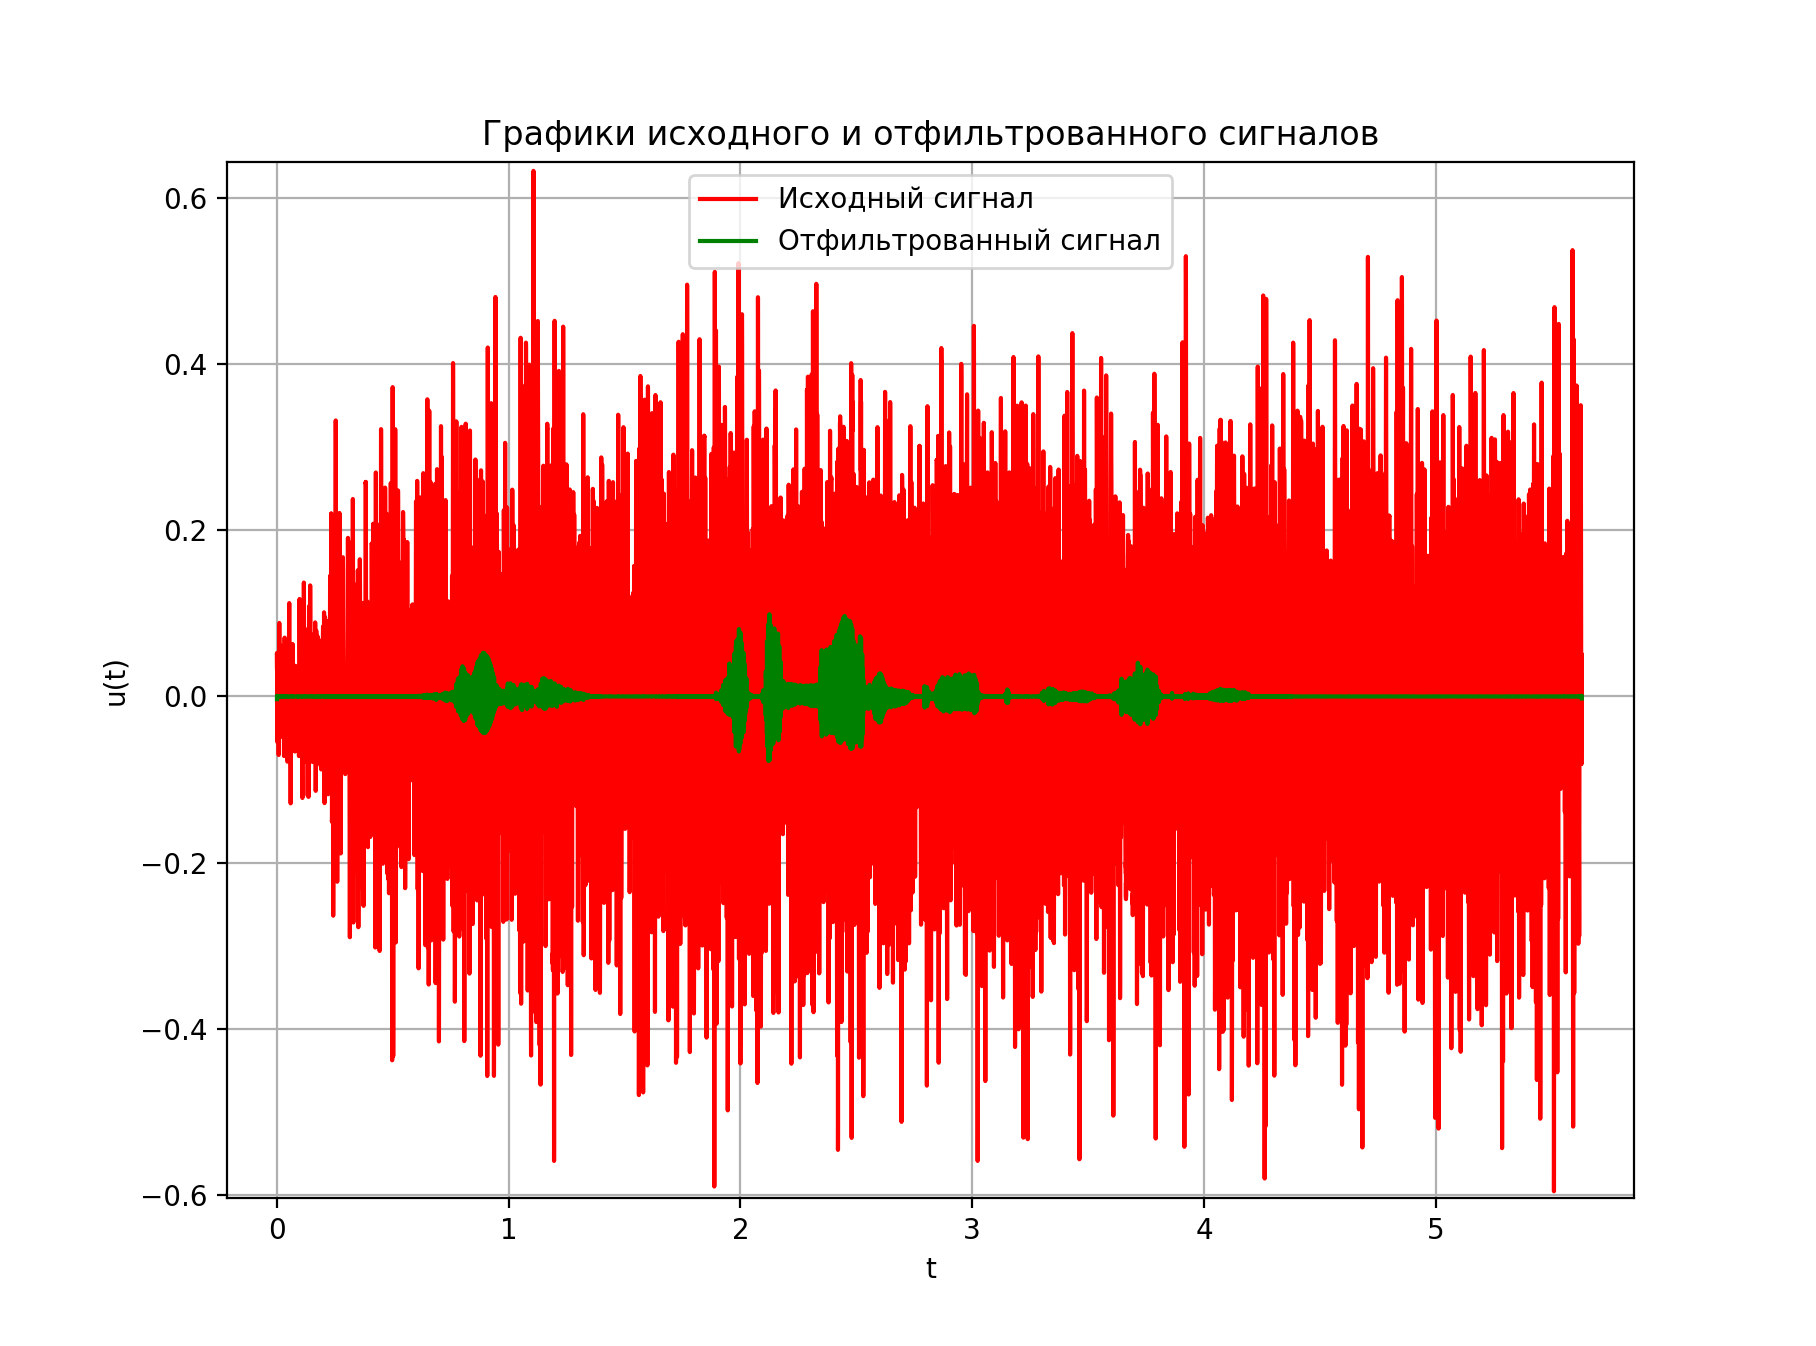
\includegraphics[scale=0.6]{media/2 task/Wave_comparison.png}
    \caption{Графики исходной и отфильтрованной звуковых волн}
    \label{fig:filteredс_wave}
\end{figure}